\documentclass[12pt]{article}
\usepackage[russian]{babel}
\usepackage{fullpage}
\usepackage[T1]{fontenc}
\usepackage[utf8]{inputenc}
\usepackage{graphicx}
\usepackage{hyperref}
%\usepackage{amsmath,amssymb}
\title{CGMIPT 2013 - Postscript Task}
\author{Денис Анисимов}
\date{}
\begin{document}
\maketitle
\section*{Реализация}
В качестве тестовой таблицы была выбрана USAF-1951. Таблица представляет собой набор групп из 6ти элементов. Каждый элемент состоит из 3х вертикальных и трёх горизонтальных полос. Относительные размеры элемента показаны на рисунке \ref{fig:elem} .

\begin{figure}[!h]
  \begin{center}
  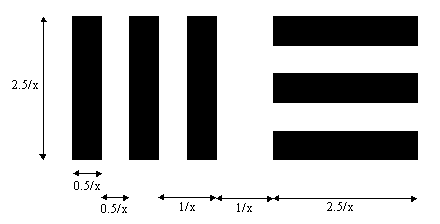
\includegraphics[scale=0.5]{USAFTestElementSpec.png}  
  \end{center}
  \caption[Элемент таблицы]{Элемент таблицы\protect\footnotemark}
  \label{fig:elem}
\end{figure}
\footnotetext{Источник:\url{http://www.efg2.com/Lab/ImageProcessing/TestTargets/}}
\end{document}